\section{Introduction}
The \ac{TCA} implementation for the \ac{CMR} is one that heavily utilizes geometry and a rigid-body model assumption, while also placing an emphasis on relying on minimal assumptions/data about the environment and avoiding computationally complex calculations on input data from sensors, cameras, etc. There were various reasons as to why some of these assumptions/choices were made and why the agreed upon implementation was deemed the best choice for the given scenario. \cite{tractl} Figure~\ref{traction_control:algorithms:scarecrow} shows a testbed version of the \ac{CMR}.

\begin{figure}[htbp]
	\centering
	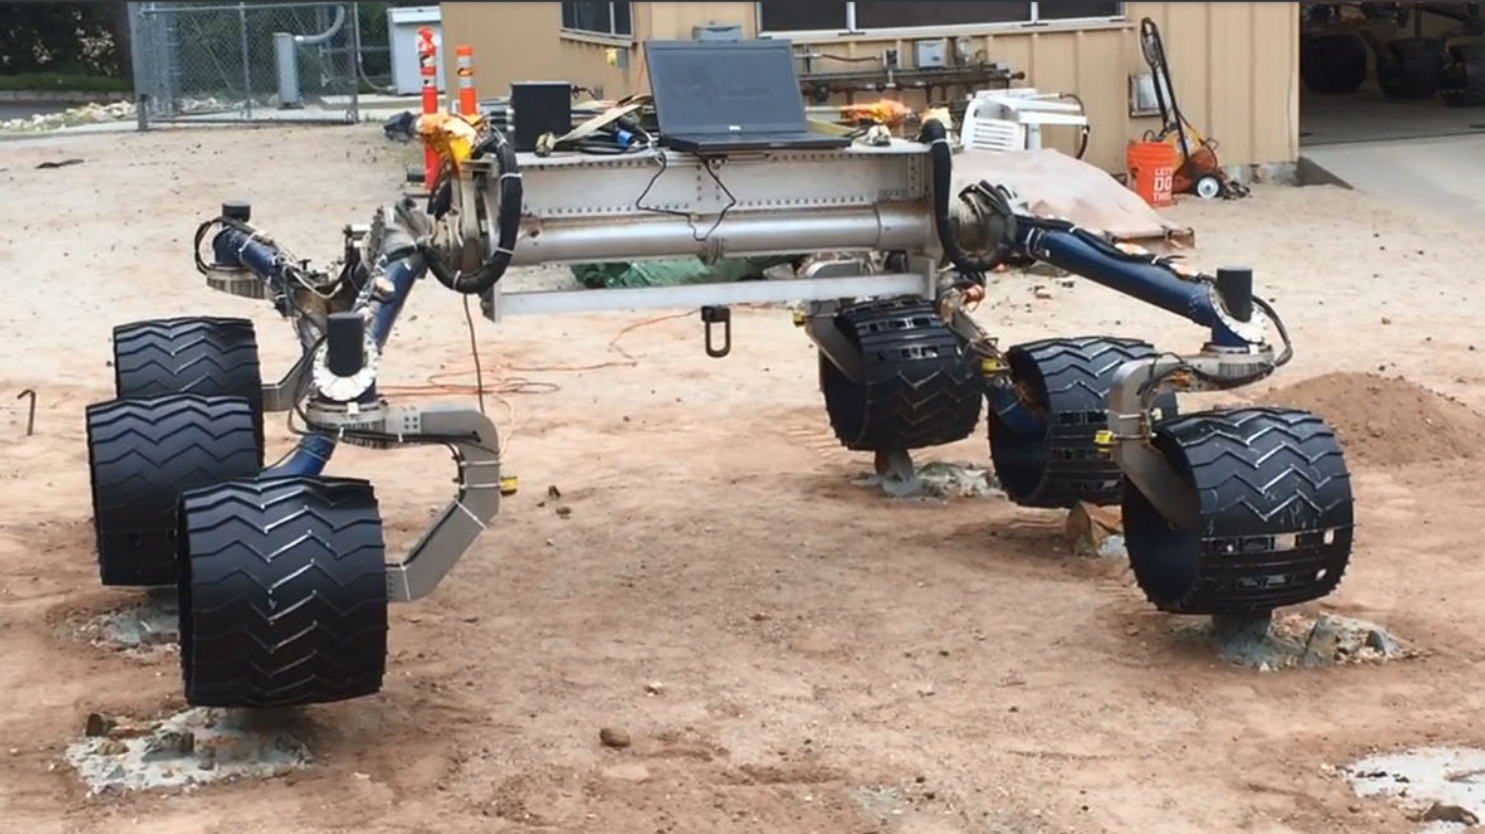
\includegraphics[width=.9\textwidth]{sections/algorithms/images/scarecrow_testbed.png}
	\caption{The Scarecrow Testbed Rover, a Rover Kinematically Similar to the \acl{CMR} \cite{tractl}}
	\label{traction_control:algorithms:scarecrow}
\end{figure}

\section{Design Limitations and Considerations}
It is important to note that the need for this \ac{TCA} was not discovered until after the flight system was actively engaging in its mission on the Martian surface, while ground control was observing telemetry of its use. Therefore, it was impossible to make any physical modifications to the \ac{CMR}, only software could be remotely flashed to it. \\

However, there are still ramifications to having this additional routine run on the \ac{CMR}. The limited computational resources available to do so must be considered carefully, so as to not interfere with existing processes being ran, and the implementation chosen has to have enough resources to perform the task it needs to as well. The team responsible for solving the problem at hand clarified some of these issues and how it restricted their choices for strategies to solve the problem. For example, the rover ``does not include force or torque sensors on the mobility subsystem, nor can it measure slip with high enough frequency to be able to react to it.'' \cite{tractl} \\

Some of the characteristics and assumptions of the \ac{CMR} and its \ac{TCA} implementation are discussed in the following sections.

\section{Ackermann Steering Model}
Modeling vehicles using the Ackermann steering model is a common practice, including for the \ac{CMR}. Even thought it adds slightly more complex geometric modeling, the mechanical steering system can be implemented relatively easily, and there are benefits to doing so. \\

Figure~\ref{traction_control:algorithms:ackermann-steering} illustrates a basic vehicle that is modeled using Ackermann steering, where the left image has the wheels positioned such that the vehicle will move straight, while the right image would cause the vehicle to turn counter-clockwise. Important to note is that when in a turning position, the front wheels are not turned to the same angle as one another, because of the nonzero distance between them. They are positioned such that the direction that both wheels are pointing are normal to a common center point called the \ac{ICC}, so that when the vehicle turns, the left and right wheels follow two different circular arcs, but both of their centers are at the \ac{ICC}.

\begin{figure}[H]
	\centering
	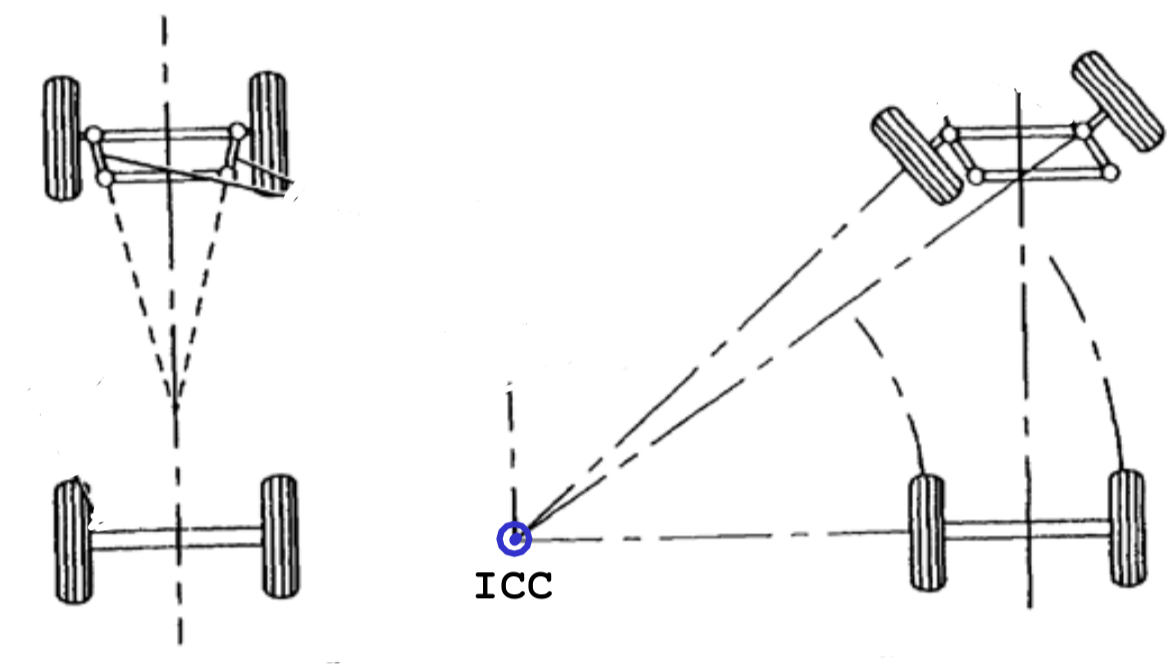
\includegraphics[width=.9\textwidth]{sections/algorithms/images/ackermann_steering.png}
	\caption{A Vehicle with Ackermann Steering Going Straight (Left) and in a Turning Position(Right)}
	\label{traction_control:algorithms:ackermann-steering}
\end{figure}

The benefit to this is that, assuming all the wheels' velocities are coordinated and in an ideal world, at no point while traveling in these flat, circular arcs will a wheel slip. Less slippage means less unpredictable behavior, such as a wheel slipping over a rough surface. However, the assumption that the \ac{CMR} would only be traversing terrain that could be modeled as flat is what led to the need for the \ac{TCA}, as excessive slippage occurred due to the reality that the terrain was non-negligible. As one wheel would traverse over a rock and then back down, it traveled a longer distance. \\

The Ackermann steering model by itself does not account for this extra distance and this caused the wheel slippage, which damaged them at an alarming rate. This is how the \ac{TCA} can be used to improve the model, so that when rough terrain is being traversed, the wheel(s) doing so can be sped up accordingly.

\section{Rigid-Body Model Assumption}\label{traction_control:algorithms:rigid-body}
The rigid-body model assumption says that a body of some sturdy material can be assumed to maintain it shape, and that a force/torque that it can expect to encounter will not deform it to a degree that needs to be accounted for. This is not true in reality, but in scenarios like these, the deformation can be negligible. \\

Making this assumption can be extremely beneficial when implementing an algorithm like \ac{TCA} because it heavily simplifies the math needed to represent vectors in different coordinate frames.

\section{Coordinate Frame Notation}\label{traction_control:algorithms:coord-frame-notation}

TO-DO, add: \\
 1.) description of what a coordinate frame is and why they're used \\
 2.) \ac{CMR} frame notation \\
 3.) mention differences in \ac{SRR} frames \\
 4.) maybe more \\

Example rotation matrix between some generic frames A and B equation:
\begin{equation}
	{}^{B}_{A}R = \left[\begin{array}{ccc}
		 \cos(\beta) & 0 & \sin(\beta) \\
		 0           & 1 & 0           \\
		-\sin(\beta) & 0 & \cos(\beta)
	\end{array}\right]
\end{equation}

The rover, like any robot, has coordinate frames to define its Denavit-Hartenburg parameters (DH) and rotation matrices. Figure~\ref{traction_control:algorithms:coordinates-side} shows these frames from the left side of the robot. A top view is also provided as Figure~\ref{traction_control:algorithms:coordinates-top}.

\begin{figure}[H]
	\centering
	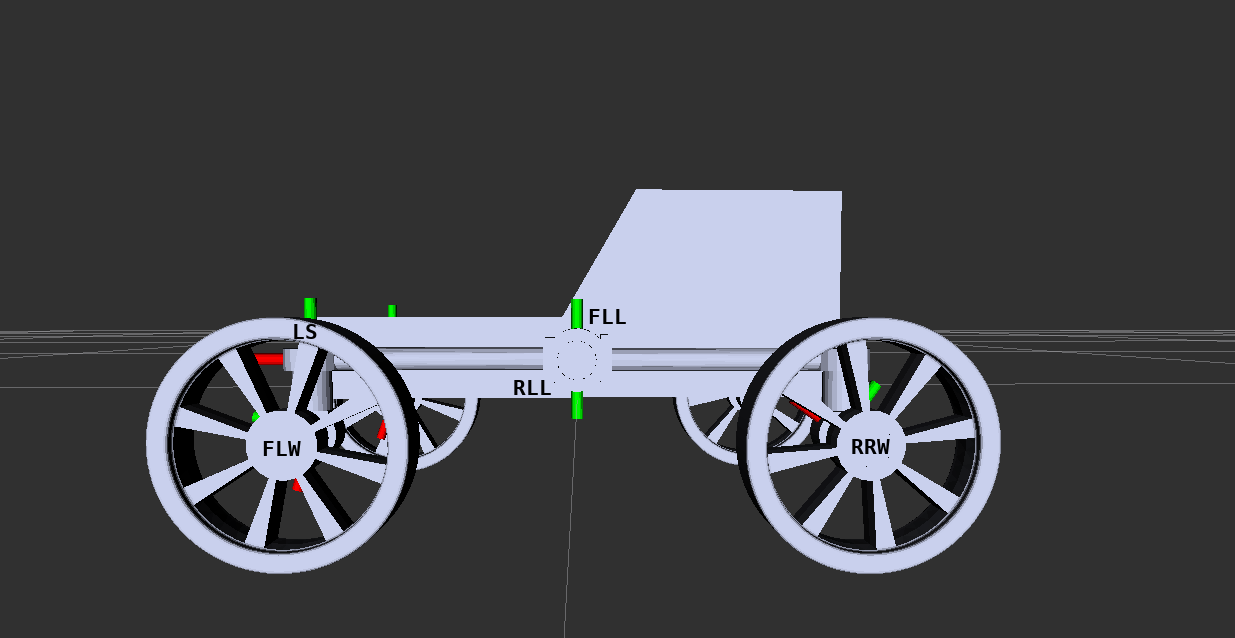
\includegraphics[width=.9\textwidth]{sections/algorithms/images/srr_side.png}
	\caption{Side View of the Robot Model and its Coordinate Frames}
	\label{traction_control:algorithms:coordinates-side}
\end{figure}
 
\begin{figure}[H]
	\centering
	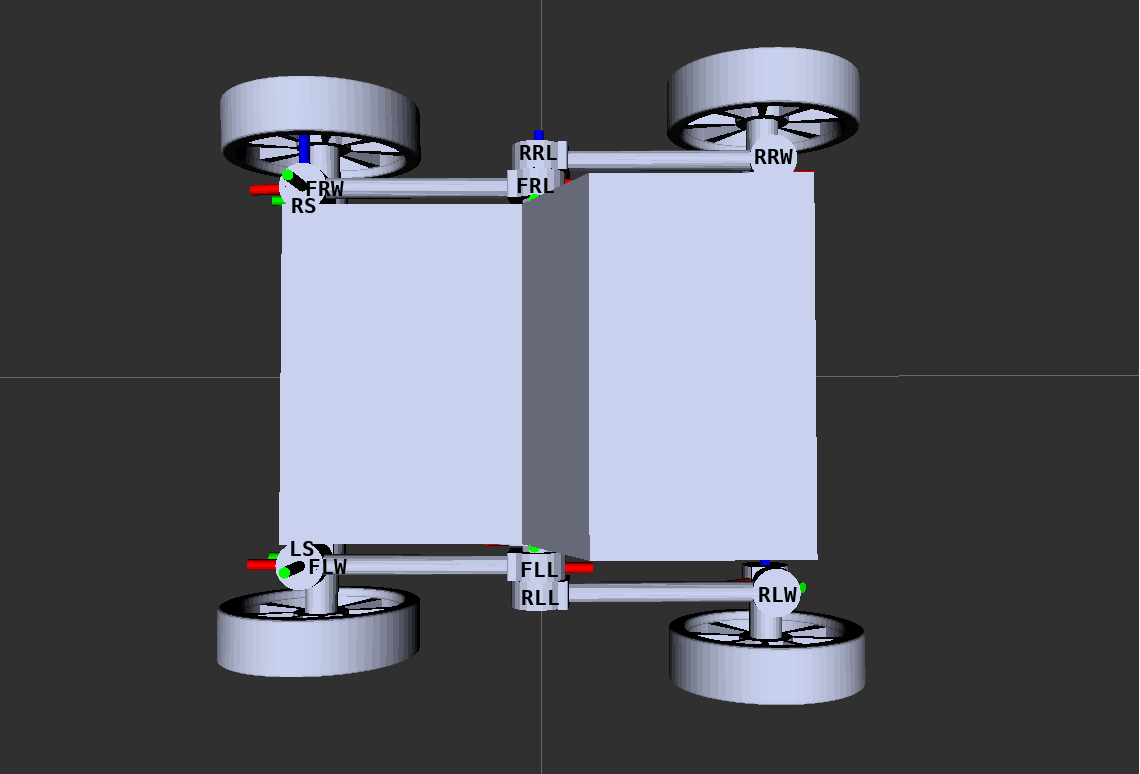
\includegraphics[width=.9\textwidth]{sections/algorithms/images/srr_top.png}
	\caption{Side View of the Robot Model and its Coordinate Frames}
	\label{traction_control:algorithms:coordinates-top}
\end{figure}
 
A summary of the acronyms for the coordinate frames used in Figures~\ref{traction_control:algorithms:coordinates-side} and~\ref{traction_control:algorithms:coordinates-top} are seen below in Table~\ref{traction_control:algorithms:frame-acronyms}.
\begin{center}\label{traction_control:algorithms:frame-acronyms}
	\begin{tabular}{rl}
		FLL & Front Left Leg \\
		FRL & Front Right Leg \\
		RLL & Rear Left Leg \\
		RRL & Rear Right Leg \\
		FLW & Front Left Wheel \\
		FRW & Front Right Wheel \\
		RLW & Rear Left Wheel \\
		RRW & Rear Right Wheel \\
		LS  & Left Steering \\
		RS  & Right Steering
	\end{tabular}
\end{center}

\section{Calculations}
\subsection{Overview}
For this algorithm on the \ac{CMR}, there are a number of configuration parameters (values that do not change throughout the lifetime of the system), a few inputs (values that are updated for each iteration of the control loop), and one output. The configuration inputs are related to the geometry of the vehicle, as that is obviously unchanging. The inputs are values such as the joint positions of the vehicle and kinematic values. The output are the ideal wheel speeds to maximize the rover's velocity while avoiding wheel slippage. These values are summarized in detail in Tables~\ref{traction_control:algorithms:inputs-cmr} and~\ref{traction_control:algorithms:outputs-cmr}.

\begin{table}[H]
	\centering
	\begin{tabular}{| >{\centering\arraybackslash}m{1.2in} | >{\centering\arraybackslash}m{4.5in} |}
		\hline
		\textbf{Input Value} & \textbf{Description} \\
		\hline
		$\left[\omega_{x}, \omega_{y}, \omega_{z}\right]^{T}$ & The 3x1 angular velocity vector around the base coordinate frame of the vehicle \\
		\hline
		$\left[\beta, \rho_{1}, \rho_{2}\right]^{T}$ & The 3x1 vector of joint positions describing the rotation of the bogie joint and each rocker joint \\
		\hline
		$\left[\dot{\beta}, \dot{\rho_{1}}, \dot{\rho_{2}}\right]^{T}$ & The 3x1 vector of angular velocities describing the rotational speed of the bogie joint and each rocker joint \\
		\hline
		$\vec{\Psi}$ & The 6x1 vector of joint positions describing the steering angle of each wheel \\
		\hline
	\end{tabular}
	\caption{Summary of the Inputs for the Traction Control Algorithm Onboard the Curiosity Mars Rover}
	\label{traction_control:algorithms:inputs-cmr}
\end{table}

\begin{table}[H]
	\centering
	\begin{tabular}{| >{\centering\arraybackslash}m{1.2in} | >{\centering\arraybackslash}m{4.5in} |}
		\hline
		\textbf{Output Value} & \textbf{Description} \\
		\hline
		$\dot{\theta}$ & The 6x1 angular velocity vector describing the ideal wheel speeds to command to the \acl{CMR} \\
		\hline
	\end{tabular}
	\caption{Summary of the Inputs for the Traction Control Algorithm Onboard the Curiosity Mars Rover}
	\label{traction_control:algorithms:outputs-cmr}
\end{table}

When considering this algorithm for the \ac{SRR}, the inputs and outputs will only change because the number of suspension joints and the number of wheels differs. The inputs and outputs for an \ac{SRR} implementation are summarized in Tables~\ref{traction_control:algorithms:inputs-srr} and~\ref{traction_control:algorithms:outputs-srr}.

\begin{table}[H]
	\centering
	\begin{tabular}{| >{\centering\arraybackslash}m{1.2in} | >{\centering\arraybackslash}m{4.5in} |}
		\hline
		\textbf{Input Value} & \textbf{Description} \\
		\hline
		$\left[\omega_{x}, \omega_{y}, \omega_{z}\right]^{T}$ & The 3x1 angular velocity vector around the base coordinate frame of the vehicle \\
		\hline
		$\vec{\delta}$ & The 4x1 vector of joint positions describing the rotation of each joint corresponding to the four legs' pivot points \\
		\hline
		$\vec{\dot{\delta}}$ & The 4x1 vector of angular velocities describing the speed of rotation of each joint corresponding to the four legs' pivot points \\
		\hline
		$\vec{\Psi}$ & The 2x1 vector of joint positions describing the steering angle of each wheel \\
		\hline
	\end{tabular}
	\caption{Summary of the Inputs for the Traction Control Algorithm Onboard the Curiosity Mars Rover}
	\label{traction_control:algorithms:inputs-srr}
\end{table}

\begin{table}[H]
	\centering
	\begin{tabular}{| >{\centering\arraybackslash}m{1.2in} | >{\centering\arraybackslash}m{4.5in} |}
		\hline
		\textbf{Output Value} & \textbf{Description} \\
		\hline
		$\dot{\theta}$ & The 4x1 angular velocity vector describing the ideal wheel speeds to command to the \acl{SRR} \\
		\hline
	\end{tabular}
	\caption{Summary of the Inputs for the Traction Control Algorithm Onboard the Curiosity Mars Rover}
	\label{traction_control:algorithms:outputs-srr}
\end{table}

\subsection{Measuring the Inputs}
As mentioned previously, one of the advantages to this implementation for traction control is that there is relatively less input data to process. Nonetheless, there are still the few inputs described in Tables~\ref{traction_control:algorithms:inputs-cmr} and~\ref{traction_control:algorithms:inputs-srr} that must be measured. \\

Each of the joints on the \ac{CMR} that appear in Table~\ref{traction_control:algorithms:inputs-cmr} have encoders that measure the current absolute position of the joint, including $\beta$, $\rho_{1,2}$, and $\Psi_{1-6}$. Some encoders are capable of measuring the current velocity of the corresponding motor as well, but the \ac{CMR} was not equipped with these. The team behind the solution in \cite{tractl} proposed instead manually computing the time derivative of the input positions to estimate each angular velocity ($\dot{\beta}$, $\dot{\rho_{1}}$, and $\dot{\rho_{2}}$). In other words, given two contiguous samples of the position of each joint, the average angular velocity over the length of time between these two samples $\Delta t$ can be calculated for some angle $\alpha$ as:

\begin{equation}
	\dot{\alpha} \approx \dot{\alpha}_{ave} = \frac{\alpha_{1} - \alpha_{0}}{\Delta t}
\end{equation}

The angular velocity vector $\dot{\omega}$ is measured with an \ac{IMU}, and more specifically with the gyroscope(s) within it. This mechanical device is a mechanism with three degrees of freedom, whose components rotate about their axes as it's turned itself. These rotations are measured as the angular velocities about those three principal axes. See Figure~\ref{traction_control:algorithms:gyro} for a 3D rendering of a gyroscope.

\begin{figure}[H]
	\centering
	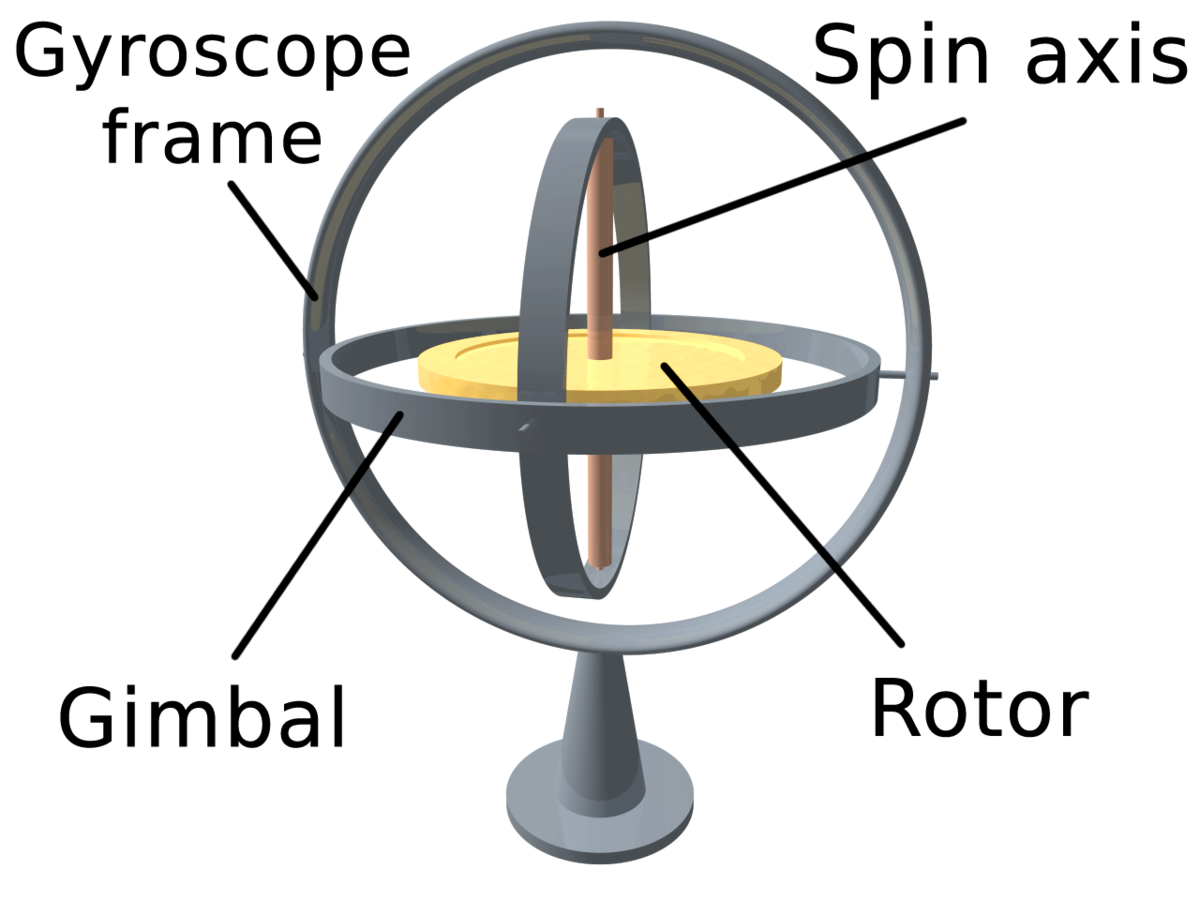
\includegraphics[width=.35\textwidth]{sections/algorithms/images/gyroscope.png}
	\caption{A 3D Rendering of a Gyroscope}
	\label{traction_control:algorithms:gyro}
\end{figure}

\subsection{Transforming Velocities Between Coordinate Frames}
To solve the problem at hand, the velocity of each wheel must be calculated in their own respective coordinate frames, which would be due to the linear and angular velocities of the vehicle, as well as then angular velocities of each of the joints of the links that connect the wheel to the chassis of the vehicle. An estimate for this velocity can be calculated once the angle between the wheel and the surface it is on is found, called the contact angle. Figure~\ref{traction_control:algorithms:wheel-frame} illustrates the velocity $\vec{v}$ and contact angle $\eta$ of a generic wheel A. \\

\begin{figure}[htbp]
	\centering
	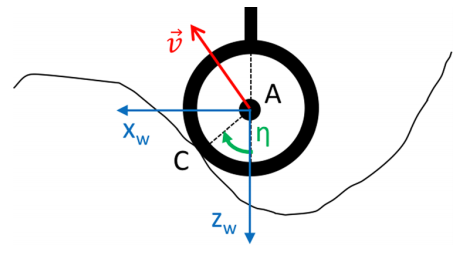
\includegraphics[width=.6\textwidth]{sections/algorithms/images/wheel_frame.png}
	\caption{The Coordinate Frame Attached to the Wheel, Illustrating the Wheel's Velocity and Contact Angle to the Surface \cite{tractl}}
	\label{traction_control:algorithms:wheel-frame}
\end{figure}

In general, the linear velocity of some point Q resolved in some coordinate frame H (which is attached to some rigid body) can be expressed as a function of some other frame G (which is attached to some other rigid body), as follows \cite{craig}:

\begin{equation}\label{traction_control:algorithms:VQG1}
	{}^{G}\vec{V}_{Q} = {}^{G}\vec{V}_{H_{0}} + ({}^{G}_{H}R \cdot {}^{H}\vec{V}_{Q}), \text{when } {}^{G}_{H}\dot{R} = I_{3}
\end{equation}

In other words, Equation~\ref{traction_control:algorithms:VQG1} states that when the rotational offset between frames G and H is constant, the linear velocity of point Q resolved in G is the sum of the linear velocity of the origin of H with respect to G and the linear velocity of Q with respect to H rotated to be resolved in G. However, it is not accurate to assume the orientation between two bodies will be static as time passes. The linear velocity of a point induced by a rotational offset that changes with time can be calculated as follows \cite{craig}:

\begin{equation}\label{traction_control:algorithms:VQG2}
	{}^{G}\vec{V}_{Q} = {}^{G}\vec{\omega}_{H} \times ({}^{G}_{H}R \cdot {}^{B}{Q}), \text{when } {}^{G}\vec{V}_{H_{0}} = {}^{H}\vec{V}_{Q} = \vec{0}_{3x1}
\end{equation}

Equation~\ref{traction_control:algorithms:VQG2} states that when the origins of frames G and H are coincident but the orientation between them changes as time passes, the linear velocity of Q resolved in frame H equals the cross product of the angular velocity between frames G and H with point Q resolved in frame G. \\

Equations~\ref{traction_control:algorithms:VQG1} and~\ref{traction_control:algorithms:VQG2} can be combined to eliminate their prior assumptions, such that:

\begin{equation}\label{traction_control:algorithms:VQG3}
	{}^{G}\vec{V}_{Q} = {}^{G}\vec{V}_{H_{0}} + ({}^{G}_{H}R \cdot {}^{H}\vec{V}_{Q}) + ({}^{G}\vec{\omega}_{H} \times ({}^{G}_{H}R \cdot {}^{B}{Q}))
\end{equation}

Equation~\ref{traction_control:algorithms:VQG3} describes how to calculate the linear velocity of a point resolved to one frame attached to a rigid body that was originally resolved to a frame attached to another rigid body. Now consider the implications of these frames being attached to a single rigid body instead. The orientation between frames G and H cannot change, because the frames rotate as the body does, implying that rotating one rotates the other in the same manner. \\

\begin{equation}\label{traction_control:algorithms:VQG4}
	{}^{G}\vec{V}_{Q} = DummyEqn.
\end{equation}

XXXXXXX \\
FINISH ME LATER \\
XXXXXXX
